\documentclass[hidelinks,11pt]{article}

\usepackage[margin=1in]{geometry}
%\usepackage{mathpazo}
\usepackage[title,titletoc,toc]{appendix}
\usepackage{multirow}
% for much better looking tables
\usepackage{booktabs} 
% tables spanning multiple pages
\usepackage{longtable}

%%% FIGURES AND FLOATS
% make it possible to include more than one captioned figure/table in a single float
\usepackage{subcaption} 
\usepackage{graphicx}
% Enables the Here Dammit figure position.
\usepackage{float} 
\usepackage{dblfloatfix}
\usepackage{fixltx2e}
\usepackage[format=plain,font=small,labelfont=bf]{caption} %caption
                                %formatting

%%% MISC
\usepackage[utf8]{inputenc}
\usepackage{blindtext}
\usepackage{color}
\usepackage{cleveref}
\usepackage[hidelinks,bookmarks]{hyperref}

% for better arrays (eg matrices) in maths
\usepackage{array} 
\usepackage{verbatim}
% nice enumerations
\usepackage{paralist} 

\usepackage{listings} % All code (looks nicer...)
\usepackage{xcolor,color}
\definecolor{mygreen}{rgb}{0,0.6,0}
\definecolor{dkgreen}{rgb}{0,0.6,0}
\definecolor{dkpurple}{rgb}{0.4,0.1,0.4}
\definecolor{blue}{rgb}{0.0,0.0,1.0}
\definecolor{light-gray}{gray}{0.9}
\definecolor{gray}{rgb}{0.5,0.5,0.5}
\definecolor{mauve}{rgb}{0.58,0,0.82}
\definecolor{green}{RGB}{0,127,0}

\lstdefinestyle{java}{ language=Java }
\lstdefinestyle{c}{ language=C }
\lstdefinestyle{python}{ language=Python }
\lstdefinestyle{makefile}{ language=[gnu]make }
\lstdefinestyle{bash}
{
  language=bash,
  backgroundcolor=\color{light-gray}
}

\lstset
{
  numbers=left, 
  firstnumber=1,
  stepnumber=1,
  numberfirstline,
  numberstyle=\scriptsize, %\sffamily
  frame=single, 
  frameround=tttt,
  tabsize=4,
  basicstyle=\small\ttfamily, 
  keywordstyle=\bfseries\color{dkpurple},
  stringstyle=\color{blue}, 
  commentstyle=\color{dkgreen}, 
  showstringspaces=false,
  aboveskip=0.5em, 
  belowskip=0em,
  captionpos=b,
  xleftmargin=1.5em,
  xrightmargin=0.5em
}

\usepackage{MnSymbol}
\lstset{prebreak=\raisebox{0ex}[0ex][0ex]
        {\ensuremath{\rhookswarrow}}}
\lstset{postbreak=\raisebox{0ex}[0ex][0ex]
        {\ensuremath{\rcurvearrowse\space}}}
\lstset{breaklines=true, breakatwhitespace=true}
%%% BIBLIOGRAPHY
\usepackage{cite}


%%% Fancy page style
\usepackage{fancyhdr} % fancy headers
\pagestyle{fancy}
\fancyhead{}

\sloppy
\frenchspacing

\renewcommand{\headrulewidth}{0.4pt}
\renewcommand{\footrulewidth}{0.4pt}
\setlength{\parindent}{0.0in}
\setlength{\parskip}{3pt}

\fancyhead{}
\fancyhead[L]{Project 4 -- Face Recognition}
\fancyhead[R]{Koch, Hart, Beckman}
\fancyfoot{}
\fancyfoot[L]{New Mexico Tech / Fall 2014 / Math 430}
\fancyfoot[R]{\thepage}

\begin{document}
\title{Project 4: Face Recognition}
\author{Christopher Koch\\David Hart\\Darrel Beckman\\
Math 430}
\maketitle

\section{Introduction}

In this project, we seeked to classify images of faces by gender using machine
learning. This was based on a face database\cite{fei} from the Centro
Universitário da FEI in Brazil, which included both smiling and non-smiling
aligned images. The algorithm developed on these images was then used on 1000
images from the Labeled Faces in the Wild database out of the University of
Massachusetts\cite{lfw}. 

\section{Model Description}

Several methods of face classification were tried. First, singular values were
obtained for both smiling and non-smiling images and it was clear that they were
approximately in the same range. However, the $k$th-rank right-singular vector
of the images was inspected and it was found that for $k = 2$, we can partition
males and females easily in a very na\"ive way. Finally, we used MATLAB's
\lstinline[language=Matlab]{classify} function with the $k$th-rank
right-singular vector of a training set to classify faces into male and female.
This \lstinline[language=Matlab]{classify} function is based on Fisher's Linear
Discriminant Analysis (LDA).

\subsection{Na\"ive Classifier}

% talk about rank-2 right-singular vector classifier, 90% accuracy? -> get data

\subsection{LDA Classifier} 

Using a training set, we create the matrix $M$ such that each column represents
one image. We then calculate
\[ \left[ U, S, V \right] = \mathrm{svd}(M) \]
and obtain the $V$ coefficients of the remaining data set $M^*$ using
\[ V^* = S \backslash (U \backslash M^*). \]

We then use MATLAB's \lstinline[language=Matlab]!classify! function, which is
based on Fisher's linear discriminant analysis \cite{classify}. Because we used
the ``diaglinear'' setting, this is a na\"ive Bayes classifier. The setting
means that the covariance matrix was diagonal and thus the input variables are
conditionally independent, which means that the classifer is na\"ive Bayes
\cite{nbayes}.

% eigenfaces!

\section{Data And Analysis}

% talk about FEI database results
% non-smiling -> smiling esp (rank-k approximation will look different because smiling, duh)
% mean faces for both FEI and LFW separately
% talk about LFW results, why not as accurate (not centered, mean image)

% graphs: accuracy vs k for LFW, same for FEI (I will generate better graphs
% than we have at the moment.)

\begin{figure}[!ht]
  \centering
  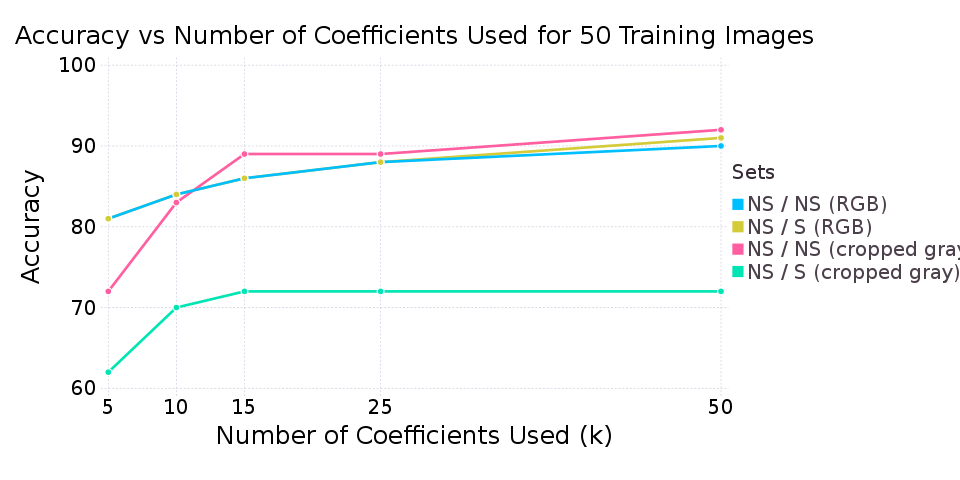
\includegraphics[width=0.8\textwidth]{accuracy_k.png}
  \caption{Accuracy vs number of coefficients used for FEI database}
  \label{fig:data:accuracy_fei}
\end{figure}

\begin{figure}[!ht]
  \centering
  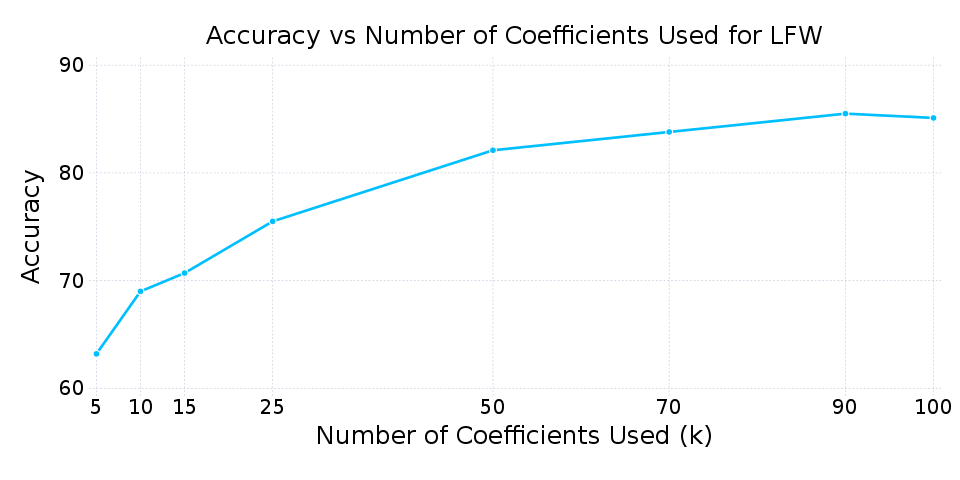
\includegraphics[width=0.8\textwidth]{accuracy_k_lfw.png}
  \caption{Accuracy vs number of coefficients used for Labeled Faces in the Wild}
  \label{fig:data:accuracy_lfw}
\end{figure}


\section{Conclusion}

A na\"ive Bayes classification system such as MATLAB's
\lstinline[language=Matlab]!classify! based on LDA is decent for classifying
gender in both non-smiling and smiling images when a training set of non-smiling
images is used. It seems plausible that such a classifier could also be used to
distinguish other physical characteristics and shapes. 

Even though the images in the Labeled Faces in the Wild were not all from the
same angle, the classifier still achieved up to 87.5\% accuracy when enough
coefficients were used. 

% talk about some future work.

% TODO: 3d surface of k vs training size vs accuracy? -> sunday morning,
% possibly
% TODO: FEI as training set on LFW? -> sunday morning

\pagebreak
\begin{appendices}
  \section{Code}
  \label{sec:app:code}

  \subsection{Classification Algorithm}
  \lstinputlisting[style=c,language=Matlab]{../classifyImages.m}

  \subsection{Image Resizing}

  \subsubsection{crop\_face.py}
  \lstinputlisting[style=c,language=Python]{../crop_face.py}

  \subsubsection{imsize.py}
  \lstinputlisting[style=c,language=Python]{../imsize.py}

  \pagebreak
  \section{Data}
  \label{sec:app:data}

  \begin{longtable}{p{6em} p{5em} p{6em} p{6em} p{6em} p{6em}}
      \toprule
      Training / Classifying & \# training images  & \# coefficient columns  & False ID as M & False
      ID as F & Accuracy \\
      \midrule
      \midrule
      \multirow{3}{6em}{Non-smiling / Non-smiling (RGB)} 
                                & 5   & 5   & 39\%  & 38\%  & 61\% \\
                                & 10  & 10  & 26\%  & 21\%  & 75\% \\
                                & 15  & 15  & 19\%  & 15\%  & 81\% \\
                                & 25  & 25  & 13\%  & 14\%  & 87\% \\
                                & 50  & 5   & 20\%  & 18\%  & 81\% \\
                                & 50  & 10  & 18\%  & 15\%  & 84\% \\
                                & 50  & 15  & 15\%  & 14\%  & 86\% \\
                                & 50  & 25  & 12\%  & 13\%  & 88\% \\
                                & 50  & 50  & 8\%   & 10\%  & \bfseries 90\% \\
      \midrule
      \multirow{3}{6em}{Non-smiling / Smiling (RGB)} 
                                & 5   & 5   & 15\%  & 22\%  & 80\% \\
                                & 10  & 10  & 17\%  & 16\%  & 81\% \\
                                & 15  & 15  & 13\%  & 14\%  & 86\% \\
                                & 25  & 25  & 11\%  & 13\%  & 88\% \\
                                & 50  & 5   & 9\%   & 14\%  & 88\% \\
                                & 50  & 10  & 11\%  & 13\%  & 88\% \\
                                & 50  & 15  & 12\%  & 12\%  & 88\% \\
                                & 50  & 25  & 11\%  & 11\%  & 89\% \\
                                & 50  & 50  & 11\%  & 9\%   & \bfseries 90\% \\
      \midrule
      \multirow{3}{6em}{Non-smiling, cropped / Non-smiling, cropped (Gray)} 
                                & 5   & 5   & 33\%  & 35\%  & 66\% \\
                                & 10  & 10  & 23\%  & 32\%  & 77\% \\
                                & 15  & 15  & 20\%  & 20\%  & 80\% \\
                                & 25  & 25  & 22\%  & 15\%  & 78\% \\
                                & 50  & 5   & 28\%  & 27\%  & 72\% \\
                                & 50  & 10  & 16\%  & 18\%  & 83\% \\
                                & 50  & 15  & 11\%  & 14\%  & 89\% \\
                                & 50  & 25  & 10\%  & 11\%  & 89\% \\
                                & 50  & 50  & 7\%   & 9\%   & \bfseries 92\% \\
      \midrule
      \multirow{3}{6em}{Non-smiling, cropped / Smiling, cropped (Gray)} 
                                & 5   & 5   & 44\%  & 32\%  & 52\% \\
                                & 10  & 10  & 37\%  & 17\%  & 62\% \\
                                & 15  & 15  & 38\%  & 13\%  & 62\% \\
                                & 25  & 25  & 31\%  & 15\%  & 68\% \\
                                & 50  & 5   & 35\%  & 28\%  & 62\% \\
                                & 50  & 10  & 29\%  & 17\%  & 70\% \\
                                & 50  & 15  & 29\%  & 15\%  & 72\% \\
                                & 50  & 25  & 33\%  & 8\%   & 72\% \\
                                & 50  & 50  & 30\%  & 12\%  & \bfseries 72\% \\
      \midrule
      \multirow{3}{6em}{Labeled Faces in the Wild, cropped}
                                & 250 & 5   & 34.6\%  & 43.6\%  & 63.2\% \\
                                & 250 & 10  & 27.1\%  & 43.1\%  & 69\% \\
                                & 250 & 15  & 26.2\%  & 38.8\%  & 70.7\% \\
                                & 250 & 25  & 21.3\%  & 34.3\%  & 75.5\% \\
                                & 250 & 50  & 14.4\%  & 28.6\%  & 82.1\% \\
                                & 250 & 70  & 9.3\%   & 34.8\%  & 83.8\% \\
                                & 250 & 90  & 8.8\%   & 30.7\%  & \bfseries 85.5\% \\
                                & 250 & 100 & 9\%     & 31.7\%  & 85.1\% \\
      \bottomrule
    \caption{Results}
    \label{tab:data}
  \end{longtable}

\end{appendices}

\pagebreak
\bibliography{IEEEabrv,proj4}
\bibliographystyle{IEEEtran}

\end{document}
